\documentclass[conference]{IEEEtran}
\usepackage{graphicx}

\title{ECG Heartbeat Classification: A Machine Learning Approach}
\author{Nguyen Son}
\begin{document}

\maketitle

\begin{abstract}
    This report is not using GPT or anything fancy, it's just a simple report about ECG Heartbeat Classification using Machine Learning. I will introduce you to the project, then I will talk about the background, the method, the results, the discussion, and the conclusion. I hope you enjoy it.
\end{abstract}

\section{Introduction}
This is the Introduction which I will write out the definition for things and introduce you to the project.

\subsection{Heart}
Heart is a pretty important organ in the human that we cannot live without. This is an essential organ in animals too. To be more scientific, a heart is a muscle that pumps blood to all parts of your body. (https://www.betterhealth.vic.gov.au/health/conditionsandtreatments/heart)

\subsection{Heartbeat}
Heartbeat is the rhythmic contraction and relaxation of heart muscles. It's like a continuous drum that's hit all the time, sometimes fast and hard, sometimes slow and calm, but if it not beat anymore, you die. (https://www.vedantu.com/evs/what-is-heartbeat)

\subsection{Heartbeat in Clinical Diagnosis}
People (Doctors mostly) can use the heartbeat to diagnose the health of a person. The heartbeat can tell you if the person is healthy or not, if the person is stressed or not, if the person is in love or not. If it not beat, you die.

\subsection{Machine Learning}
It's the use and development of computer systems that are able to learn and adapt without following explicit instructions, by using algorithms and statistical models to analyze and draw inferences from patterns in data. (Oxford Dictionary)

\subsection{Machine Learning in Heartbeat Classification}
It's the use and development of computer systems that are able to learn and adapt without following explicit instructions, by using algorithms and statistical models to analyze and draw inferences from patterns in people's heartbeat for classification. (me, i guess)

\subsection{What others do in Machine Learning for Heartbeat Classification}
It takes time to do this, so I will do it later (hopefully).

\subsection{State Problem}
This is necessary, so we need to do this!!1!!

\section{Background}
\subsection{ECG}
An electrocardiogram records the electrical signals in the heart. It's a common and painless test used to quickly detect heart problems and monitor the heart's health. (https://www.mayoclinic.org/tests-procedures/ekg/about/pac-20384983)

\subsection{CNN}
A Convolutional Neural Network, also known as CNN or ConvNet, is a class of neural networks that specializes in processing data that has a grid-like topology, such as an image. A digital image is a binary representation of visual data. It contains a series of pixels arranged in a grid-like fashion that contains pixel values to denote how bright and what color each pixel should be. (https://towardsdatascience.com/convolutional-neural-networks-explained-9cc5188c4939)

\section{Method}
I use Random Forest Model. It's a good model.

First I load the data, then I preprocess the data, then I train the model, then I evaluate the model.

\section{Results}
I don't know how to make a table in LaTeX, so here is a screenshot instead.
\begin{figure}[h]
    \centering
    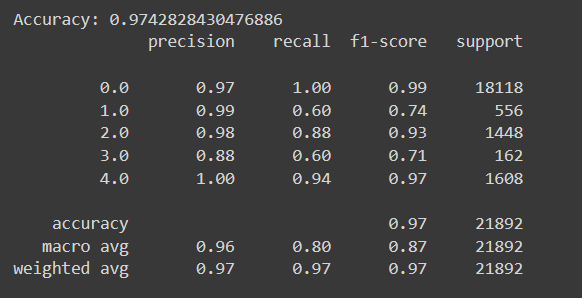
\includegraphics[width=\linewidth]{accuracy.png}
    \caption{Accuracy}
    \label{fig:accuracy}
\end{figure}

and here is the confusion matrix:

\begin{figure}[h]
    \centering
    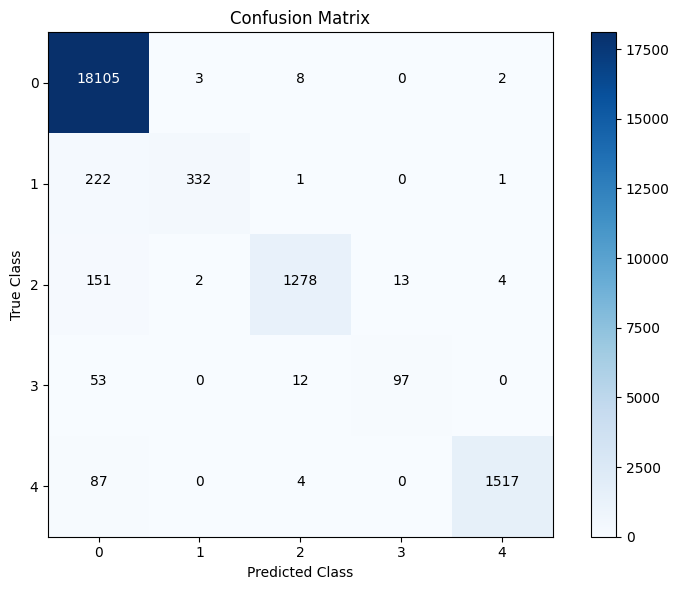
\includegraphics[width=\linewidth]{confusionmatrix.png}
    \caption{Confusion Matrix}
    \label{fig:accuracy}
\end{figure}

\section{Discussion}
It's pretty good I suppose?

\section{Conclusion}
Yay I'm done with the first practial let me go to sleep now.

\end{document}
